%//==============================--@--==============================//%
\subsection[3.4 Reliable Data Transfer]{\hspace*{0.075 em}\raisebox{0.2 em}{$\pmb{\drsh}$} Reliable Data Transfer}
\label{subsec:reliable-data-transfer}

%//==============================--@--==============================//%
\subsubsection[3.4.1 Stop-and-Wait]{\hspace*{0.075 em}\raisebox{0.2 em}{$\pmb{\rightarrow}$} Stop-and-Wait}
\label{subsec:stop-and-wait}

Stop-and-wait is a simple and fundamental technique for reliable data transfer. The sender transmits a single data packet and then waits for an acknowledgment (ACK) from the receiver before transmitting the next packet.

\vspace{-0.5em}
\begin{enumerate}
    \item \textbf{Packet numbering}: To detect and discard duplicate packets, both data packets and ACKs are numbered. The receiver can then distinguish between new packets and duplicates.
    
    \item \textbf{Error detection}: Both data packets and ACKs include a checksum for error detection. If the receiver detects an error in a packet, it discards the packet without sending an ACK, prompting the sender to retransmit the packet.
    
    \item \textbf{Timeout and retransmission}: The sender sets a timer after transmitting a packet. If the timer expires before receiving an ACK, the sender assumes the packet or the ACK was lost and retransmits the packet.
\end{enumerate}

\begin{quote}
    ``If we define the utilization of the sender (or the channel) as the fraction of time the sender is actually busy sending bits into the channel, $[$direct observation$]$ (...) shows that the stop-and-wait protocol has a rather \textbf{dismal sender utilization} (...)''\cite{Kurose2017}
    $$
        U_\text{sender} = \frac{L/R}{\text{RTT} + L/R} \ll 1
    $$
\end{quote}

\noindent The solution to this \textit{conundrum} is known as \textbf{pipelining} as discussed bellow, where two basic approaches toward pipelined error recovery can be identified.

%//==============================--@--==============================//%
\subsubsection[3.4.2 Cumulative ACKs and Selective ACKs]{\hspace*{0.075 em}\raisebox{0.2 em}{$\pmb{\rightarrow}$} Cumulative ACKs and Selective ACKs}
\label{subsec:cumulative-acks-selective-acks}

\vspace{-0.5em}
\begin{enumerate}
    \item \textbf{Cumulative ACKs}: In this approach, the receiver acknowledges the receipt of all consecutive, correctly received packets up to a specified sequence number by sending an \underline{ACK containing the sequence number of the next expected packet}. If a packet is lost or arrives out of order, the receiver sends an ACK with the sequence number of the first expected packet it has not received.
    
    \item \textbf{Selective ACKs}: With selective ACKs, the receiver explicitly acknowledges \underline{individual packets}, allowing the sender to retransmit only the missing packets. This approach improves efficiency, especially in scenarios with high packet loss or long round-trip times.
\end{enumerate}

%//==============================--@--==============================//%
\subsubsection[3.4.3 Sliding Window Protocol]{$\pmb{\rightarrow}$ Sliding Window Protocol}

The sliding window protocol is a general concept that forms the basis for both Go-Back-N (GBN) and Selective Repeat (SR) protocols. It allows the sender to transmit multiple packets without waiting for an acknowledgment (ACK) for each one. The sender maintains a sending window that limits the number of unacknowledged packets, while the receiver maintains a receiving window that limits the number of out-of-order packets it can accept. The windows slide as the sender receives ACKs and the receiver receives in-order packets.
$$
    \text{\underline{Relação temporal fundamental:}} \quad \boxed{\frac{L}{c} \ll \text{RTT} < W \cdot \frac{L}{c} < Timeout}
$$

\begin{figure}[H]
    \centering
    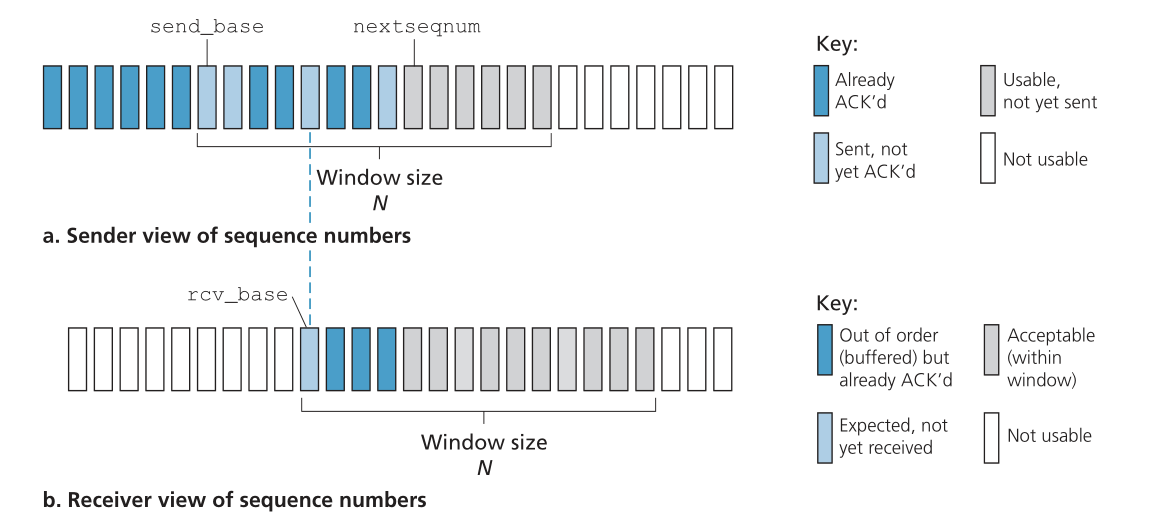
\includegraphics[width = 0.9\linewidth]{img/3/send-and-receive-windows.png}
    \caption{Exemplo janela deslizante}
    \label{fig:send-and-receive-windows}
\end{figure}

\paragraph[3.4.3.1 Go-Back-N (GBN)]{$\pmb{\star}$ Go-Back-N (GBN)}\mbox{}\\[4pt]
Go-Back-N (GBN) is a specific implementation of the sliding window protocol where the receiver sliding window has a size of 1. It uses a \underline{cumulative acknowledgment scheme}. If a packet is lost or corrupted, the receiver discards all out-of-order packets received after the lost packet. When the sender detects the loss, it retransmits the lost packet and all subsequent packets. GBN is relatively simple to implement, but its performance degrades in networks with high error rates, as it requires retransmission of multiple packets even if only a single packet was lost.
$$
    \text{\underline{Tamanho máximo da janela para evitar ambiguidades na receção:}} \quad \boxed{W_s \leq N_\text{seq} - 1}
$$

\paragraph[3.4.3.2 Temporizador/janela e ACKs cumulativos]{$\pmb{\star}$ Temporizador/janela e ACKs cumulativos}\mbox{}\\[4pt]
Uma alternativa ao protocolo GBN é a utilização de uma janela de tamanho igual à sender window no lado do receiver. Deste modo, a retransmissão de todos os pacotes subsequentes é evitada.
$$
    \text{\underline{Tamanho máximo da janela para evitar ambiguidades na receção:}} \quad \boxed{W \leq \left\lfloor N_\text{seq}/2 \right\rfloor}
$$

\paragraph[3.4.3.3 Selective Repeat (SR). Temporizador/pacote e ACKs seletivos]{$\pmb{\star}$ Selective Repeat (SR). Temporizador/pacote e ACKs seletivos}\mbox{}\\[4pt]
Selective Repeat (SR) is another implementation of the sliding window protocol, which addresses the performance issues of GBN. Instead of using cumulative ACKs, the receiver sends \underline{individual ACKs (selective ACKs)} for each received packet, regardless of their order. The receiver stores out-of-order packets in a buffer until the missing packets arrive. The sender only retransmits the lost or corrupted packets, which are identified by the absence of their respective ACKs. Although SR is more efficient than GBN in handling packet losses, it is more complex to implement due to the need to handle individual ACKs and maintain the buffer for out-of-order packets.
$$
    \text{\underline{Tamanho máximo da janela para evitar ambiguidades na receção:}} \quad \boxed{W \leq \left\lfloor N_\text{seq}/2 \right\rfloor}
$$

%//==============================--@--==============================//%
\subsubsection[3.4.4 Fast Retransmission with 3 ACKs]{\hspace*{0.075 em}\raisebox{0.2 em}{$\pmb{\rightarrow}$} Fast Retransmission with 3 ACKs}
\label{subsec:fast-retransmission}

Fast retransmission is an optimization technique to improve the performance of reliable data transfer protocols. It allows the sender to detect and retransmit lost packets faster than relying solely on timeouts.

\vspace{-0.5em}
\begin{enumerate}
    \item \textbf{Duplicate ACKs}: When the receiver detects an out-of-order packet, it sends a duplicate ACK sends an ACK with the sequence number of the first expected packet it has not received. The sender can infer that a packet was lost if it receives multiple duplicate ACKs.
    
    \item \textbf{Three-duplicate-ACKs rule}: If the sender receives three duplicate ACKs for the same packet, it assumes the packet was lost and immediately retransmits it without waiting for the timeout.
\end{enumerate}

%//==============================--@--==============================//%
\subsubsection[3.4.5 Reminder]{\hspace*{0.075 em}\raisebox{0.2 em}{$\pmb{\rightarrow}$} Reminder}
\label{subsec:reminder}

\paragraph[3.4.5.1 Canal não sequencial]{$\pmb{\star}$ Canal não sequencial}\mbox{}\\[4pt]
\noindent Mediante um canal não fiável não sequencial, o espaço de numeração deve ser tal que não existam repetições de identificadores dentro do intervalo de tempo decorrido entre a recepção do pacote mais rápido e a recepção do pacote mais lento, sendo o pacote mais lento emitido imediatamente antes do mais rápido:
$$
    \boxed{\text{número de identificadores} \ge r \cdot T}
$$
\noindent Onde $r$ é o débito a que os números de sequência são consumidos (1/delay de transmissão para \textit{sliding window protocol} e 1/RTT para \textit{stop-and-wait protocol}) e $T$ é o tempo de vida máxima de um pacote no canal.

\paragraph[3.4.5.2 Transmissão sem interrupção]{$\pmb{\star}$ Transmissão sem interrupção}\mbox{}
$$
    \boxed{ N_\text{pkt}\, t_\text{trans} \ge \text{RTT} + t_\text{trans} }
$$
%//==============================--@--==============================//%
\newpage
\subsubsection[3.4.5 TL;DR Reliable Data Transfer]{\hspace*{0.075 em}\raisebox{0.2 em}{$\pmb{\rightarrow}$} TL;DR Reliable Data Transfer}
\label{subsec:TLDR}

{
\setlength{\tabcolsep}{16pt}

\begin{table}[h!]
    \centering
    \captionsetup{justification=centering}
    \begin{tabularx}{\textwidth}{lX}
        \toprule
        \multicolumn{1}{c}{\textbf{Mechanism}} & \multicolumn{1}{c}{\textbf{Use, Comments}} \\
        \midrule
        Checksum & Used to detect bit errors in a transmitted packet. \\ \midrule
        Sequence number & Used for sequential numbering of packets of data flowing from sender to receiver. Gaps in the sequence numbers of received packets allow the receiver to detect a lost packet. Packets with duplicate sequence numbers allow the receiver to detect duplicate copies of a packet. \\ \midrule
        Acknowledgment & Used by the receiver to tell the sender that a packet or set of packets has been received correctly. Acknowledgments will typically carry the sequence number of the packet or packets being acknowledged. Acknowledgments may be individual or cumulative, depending on the protocol. \\ \midrule
        Negative acknowledgment & Used by the receiver to tell the sender that a packet has not been received correctly. Negative acknowledgments will typically carry the sequence number of the packet that was not received correctly. \\ \midrule
        Window, pipelining & The sender may be restricted to sending only packets with sequence numbers that fall within a given range. By allowing multiple packets to be transmitted but not yet acknowledged, sender utilization can be increased over a stop-and-wait mode of operation. We’ll see shortly that the window size may be set on the basis of the receiver’s ability to receive and buffer messages, or the level of congestion in the network, or both. \\
        \bottomrule
    \end{tabularx}
    \caption{``Summary of reliable data transfer mechanisms and their use''\cite{Kurose2017}}
    \label{tab:TLDR}
\end{table}
}

%//==============================--@--==============================//%